\documentclass[a4paper,11pt]{report}
\usepackage[slovene]{babel}
\usepackage{listings}
\usepackage{graphicx}
\usepackage[section]{placeins}

\lstset{
numberstyle=\small, 
numbersep=8pt, 
frame = single, 
language=SQL, 
framexleftmargin=15pt}

\begin{document}

\title{TUP: 5. domača naloga}
\author{Jakob Marušič}
\maketitle

\section*{Naloga (a)}

\paragraph{Navodila}
\begin{em}
    V svoji dosedanji medicinski bazi iz predhodnih domačih nalog si izberite najmanj tri tabele, najbolje takšne, ki implementirajo povezavo mnogo proti mnogo. Vsaka od tabel mora imeti najmanj 10 smiselnih vrstic. Prikažite shemo izbranih tabel in najmanj 10 vnešenih vrednosti.
\end{em}

\paragraph{Shema izbranih tabel}\mbox{}

\noindent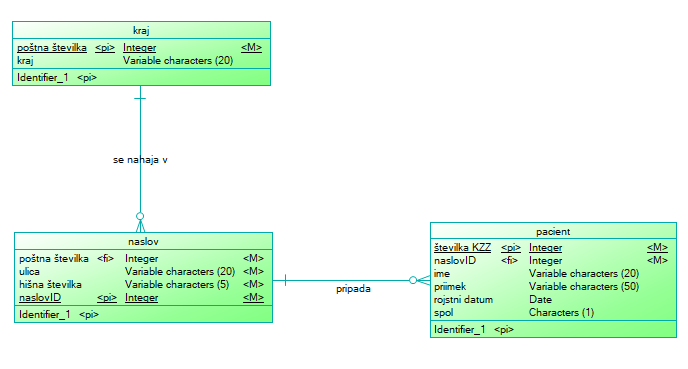
\includegraphics[width=\linewidth]{./pics/konceptualni.png}

\paragraph{Podatki v kraj}\mbox{}

\begin{tabular}{||c|c||}
    \hline
    Poštna številka&Kraj\\
    \hline
    \hline
        1000&Ljubljana\\
        2000&Maribor\\
        5000&Nova Gorica\\
        6000&Koper\\
        6223&Komen\\
        5291&Miren\\
        1001&Ljubljana\\
        1002&Ljubljana\\
        1003&Ljubljana\\
        1004&Ljubljana\\
    \hline
\end{tabular}

\pagebreak
\paragraph{Podatki v ulica}\mbox{}

\begin{tabular}{||c|c|c|c||}
    \hline
    NaslovID&Poštna številka&Ulica&Hišna številka\\
    \hline\hline
        1&1000&Svetčeva&9 \\
        2&1000&Večna pot&113 \\
        3&5000&Ulica padlih borcev&13 \\
        4&6000&Ulica s palmami&11 \\
        5&1002&Zokijeva promenada&4b \\
        6&6223&Komen&5f \\
        7&5291&Bilje&45 \\
        8&2000&Maribor Čuj&1 \\
        9&2000&Šampionska&23c \\
        10&5291&Opatje selo&2ž \\
    \hline
\end{tabular}

\paragraph{Podatki v pacient}\mbox{}

\begin{tabular}{||c|c|c|c|c|c||}
    \hline
    Številka KZZ&NaslovID&Ime&Priimek&Datum rojstva&Spol\\
    \hline\hline
        10001&1&Milo&Milovan&01.01.2001&M\\
        10005&2&Aligator&Bine&15.04.1974&M\\
        10002&3&Osama&Obama&11.09.2001&M\\
        10008&4&Cvetka&Odpoldeta&11.07.2006&Ž\\
        10009&5&Ana&Šprjtova&26.09.1931&Ž\\
        10010&6&Mino&Moka&29.02.2000&Ž\\
        10007&7&Milka&Krava&12.10.1998&Ž\\
        10006&8&Cilka&Bilka&19.03.1742&Ž\\
        10004&9&Klementina&Pomarančka&13.06.1965&Ž\\
        10003&10&Simon&Zavadlavov&12.05.1970&M\\
    \hline
\end{tabular}

\section*{Naloga (b)}

\paragraph{Navodila}
\begin{em}
    Izdelajte skripto SQL2NoSQL.py, ki se bo povezala na vašo relacijsko bazo in bo za izbrane tabele iz prvega dela ustvarila ustrezno strukturo v NoSQL bazi MongoDB ali Neo4j, ter prekopirala podatke.
\end{em}

\paragraph{Koda}\mbox{}

\begin{lstlisting}[showstringspaces=false][language = Python]
    import mysql.connector
    from pymongo import MongoClient
    import sys
    
    
    #povaezava na MongoDB bazo
    mongoClient  = MongoClient()
    mongoDB = mongoClient.tup_naloga5
    
    #povezava na MySQL bazo
    cnx = mysql.connector.connect(
        user = 'root',
        database = 'naloga5'
    )
    cursor = cnx.cursor()
    
    
    try:
        mongoDB.kraj.drop()
        mongoDB.naslov.drop()
        mongoDB.pacient.drop()
    except:
        print("Neki neki")
    
    
    collection = mongoDB.kraj
    query = "SELECT * FROM kraj"
    cursor.execute(query)
    cus = dict()
    
    id = 1
    for row in cursor:
        cus['_id'] = id
        cus['posta'] = row[0]
        cus['kraj'] = row[1]
        print(collection.insert_one(cus).inserted_id)
        id += 1
    
    
    collection = mongoDB.naslov
    query = "SELECT * FROM naslov"
    cursor.execute(query)
    cus = dict()
    
    for row in cursor:
        cus['posta'] = row[0]
        cus['ulica'] = row[1]
        cus['hisna_stevilka'] = row[2]
        cus['_id'] = row[3]
        print(collection.insert_one(cus).inserted_id)
    
    
    collection = mongoDB.pacient
    query = "SELECT * FROM pacient"
    cursor.execute(query)
    cus = dict()
    
    id = 1
    for row in cursor:
        print(row)
        cus ['_id'] = id
        cus['kzz'] = row[0]
        cus['naslovID'] = row[1]
        cus['ime'] = row[2]
        cus['priimek'] = row[3]
        cus['rojstni_datum'] = row[4]
        cus['spol'] = row[5]
        print(collection.insert_one(cus).inserted_id)
        id += 1
\end{lstlisting}

\pagebreak
\section*{Naloga (c)}

\paragraph{Navodila}
\begin{em}
    V jeziku SQL napišite poizvedbo, ki izpiše vse povezane vrednosti iz izbranih tabel. Enake rezultate na ustrezen način pridobite iz baze MongoDB ali Neo4j,in izpišite vrednosti na enak način.
\end{em}

\paragraph{SQL poizvedba}\mbox{}

\begin{lstlisting}[showstringspaces=false][language = Python]
    #SQL query
    query = "\
        select \
            p.ime, \
            p.priimek, \
            n.ulica, \
            n.hisna_stevilka, \
            k.kraj, \
            k.posta \
        from \
            pacient p \
        left join naslov n on p.naslovID = n.naslovID \
    left join kraj k on n.posta = k.posta"
    
    cursor.execute(query)
    for row in cursor:
        print(f"\
                {row[0]}\t\
                {row[1]}\t\
                {row[2]}\t\
                {row[3]}\t\
                {row[4]}\t\
                {row[5]}"
            )
\end{lstlisting}

\pagebreak
\paragraph{MongoDB poizvedba}\mbox{}

\begin{lstlisting}[showstringspaces=false][language = Python]
    rez = mongoDB.naslov.aggregate([{
        "$lookup": {
            "from": "pacient",
            "localField": "naslovID",
            "foreignField": "naslovID",
            "as": "pacient"
        }
        }, {
            "$unwind": {
                "path": "$pacient"
            }
        }, {
            "$lookup": {
                "from": "kraj",
                "localField": "posta",
                "foreignField": "posta",
                "as": "kraj"
            }
        }, {
            "$unwind": {
                "path": "$kraj"
            }
        }
    ])
    
    for doc in rez:
        print(f"\
                {doc['pacient']['ime']}\t\
                {doc['pacient']['priimek']}\t\
                {doc['ulica']}\t\
                {doc['hisna_stevilka']}\t\
                {doc['kraj']['posta']}\t\
                {doc['kraj']['kraj']}"
            )
\end{lstlisting}

\paragraph{Razlike med poizvedbami}
Iz zgoraj navedenih skript je očitno, da je sintaksa obeh poizvedb popolnoma drugačna. 
Največja težava pri pisanju MongoDB je bilo povezavanje tabel.

\end{document}